\section{Evaluation}
\label{sec:evaluation}

% Results figures, rendered from the persisted artifacts:
% bootstrap_ci.json (suite means and 95% CIs), stability_run1_vs_run2.json (run pairs).
% Values resolve through figures/generated_values.tex, which scripts/gen_sp_figures.py
% writes from those artifacts; run `python scripts/gen_sp_figures.py --check` to prove
% this figure still agrees with them.
% Layout discipline: the top panel shows point estimates + intervals only
% (no filled bars under the whiskers), the bottom panel's legend lives
% below the axis (never over the bars), and both panels share the same
% value range so the stacked scales read as one.
% GENERATED by scripts/gen_sp_figures.py -- do not edit by hand.
% Every plotted number in the S&P figures resolves through this file, so a
% figure cannot silently disagree with the artifact it claims to show.
% Regenerate:  python scripts/gen_sp_figures.py
% Verify:      python scripts/gen_sp_figures.py --check
% Sources:
%   results/bootstrap_ci.json
%   results/stability_run1_vs_run2.json
%   results/b4_baseline_zodiac_20260922.json
%   results/model_quality/chrollo_calibration.json
%   results/sp2027_rescue/behavior_trajectory_benchmark.json

\def\RaginLiveTechnique{0.9598}
\def\RaginLiveTechniqueErrLo{0.0122}
\def\RaginLiveTechniqueErrHi{0.0122}
\def\RaginLiveActor{0.8500}
\def\RaginLiveActorErrLo{0.0000}
\def\RaginLiveActorErrHi{0.0000}
\def\RaginLivePersona{0.7325}
\def\RaginLivePersonaErrLo{0.0587}
\def\RaginLivePersonaErrHi{0.0558}
\def\RaginLiveComposite{0.8796}
\def\RaginLiveCompositeErrLo{0.0224}
\def\RaginLiveCompositeErrHi{0.0204}
\def\RaginLivePersonaRunTwo{0.7504}
\def\RaginLiveCompositeRunTwo{0.8845}
\def\RaginPersonaRunDelta{0.018}
\def\RaginTechDelta{0.317}
\def\RaginTechDeltaLo{0.162}
\def\RaginTechDeltaHi{0.480}
\def\RaginActorDelta{0.140}
\def\RaginActorDeltaLo{0.083}
\def\RaginActorDeltaHi{0.197}
\def\RaginPersonaNullDelta{0.005}
\def\RaginPersonaNullDeltaLo{-0.047}
\def\RaginPersonaNullDeltaHi{0.057}
\def\RaginOverallDelta{0.154}
\def\RaginOverallDeltaLo{0.092}
\def\RaginOverallDeltaHi{0.221}
\def\RaginGroundingTtpCount{35}
\def\RaginNoGroundingTtpCount{0}
\def\RaginRoutingBefore{0.8875}
\def\RaginRoutingAfter{0.955}

\begin{figure}[t]
\centering
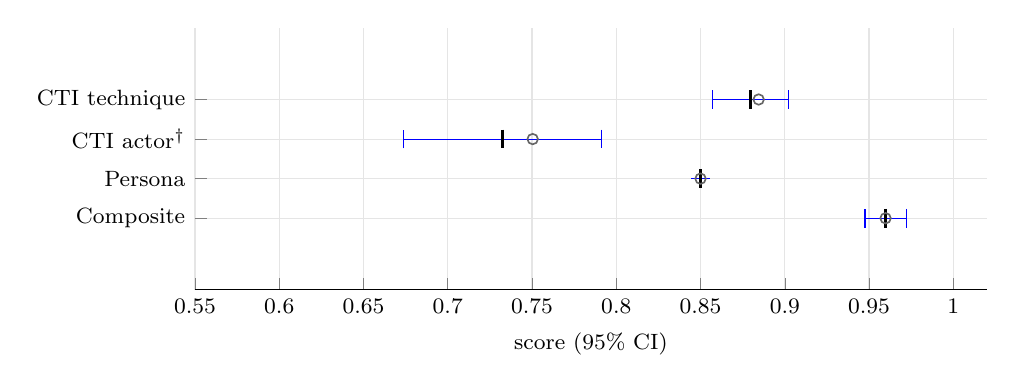
\begin{tikzpicture}
\begin{axis}[
  name=ax1,
  width=0.96\linewidth,
  height=4.9cm,
  xmin=0.55, xmax=1.02,
  y axis line style={draw=none},
  axis x line*=bottom,
  axis y line*=left,
  ytick=data,
  yticklabels={Composite,Persona,CTI actor$^{\dagger}$,CTI technique},
  y dir=reverse,
  xlabel={score (95\% CI)},
  xlabel style={font=\footnotesize},
  tick label style={font=\footnotesize},
  enlarge y limits=0.6,
  grid=major,
  grid style={black!10},
  clip=false
]
% point estimates and bootstrap 95% CIs from bootstrap_ci.json;
% only marks + intervals: no bars beneath the whiskers
\addplot+[only marks, mark=|, mark size=3.4, mark options={thick,black},
  error bars/.cd, x dir=both, x explicit] coordinates {
  (\RaginLiveTechnique,3) +- (\RaginLiveTechniqueErrLo,\RaginLiveTechniqueErrHi)
  (\RaginLiveActor,2) +- (\RaginLiveActorErrLo,\RaginLiveActorErrHi)
  (\RaginLivePersona,1) +- (\RaginLivePersonaErrLo,\RaginLivePersonaErrHi)
  (\RaginLiveComposite,0) +- (\RaginLiveCompositeErrLo,\RaginLiveCompositeErrHi)
};
% run-2 overlay: open markers (point estimates from stability_run1_vs_run2.json;
% per-suite CIs were not computed for run 2, so none are drawn)
\addplot+[only marks, mark=o, mark size=1.9, mark options={semithick,black!60}] coordinates {
  (\RaginLiveTechnique,3)
  (\RaginLiveActor,2)
  (\RaginLivePersonaRunTwo,1)
  (\RaginLiveCompositeRunTwo,0)
};
\end{axis}
\end{tikzpicture}

\vspace{2mm}

\begin{tikzpicture}
\begin{axis}[
  name=ax2,
  width=0.96\linewidth,
  height=4.9cm,
  ybar=1.5pt,
  bar width=9pt,
  ymin=0.55, ymax=1.0,
  symbolic x coords={CTI technique,CTI actor,Persona,Composite},
  xtick=data,
  ylabel={mean score},
  ylabel style={font=\footnotesize},
  tick label style={font=\footnotesize},
  ymajorgrids,
  grid style={black!10},
  enlarge x limits=0.25,
  legend style={font=\scriptsize, at={(0.5,-0.16)}, anchor=north, legend columns=2, draw=none, fill=none},
  legend cell align={left},
]
% run 1 vs run 2 from stability_run1_vs_run2.json
\addplot+[black!35, fill=black!35] coordinates {
  (CTI technique,\RaginLiveTechnique) (CTI actor,\RaginLiveActor) (Persona,\RaginLivePersona) (Composite,\RaginLiveComposite)
};
\addplot+[black!70, fill=black!70, pattern=north east lines] coordinates {
  (CTI technique,\RaginLiveTechnique) (CTI actor,\RaginLiveActor) (Persona,\RaginLivePersonaRunTwo) (Composite,\RaginLiveCompositeRunTwo)
};
\legend{run 1, run 2}
\end{axis}
\end{tikzpicture}
\caption{Live-campaign results from the persisted artifacts (identical
deterministic-strata bars across runs are the finding, not a plotting
error). All four plotted values are the \emph{both-channel} operational
score of Table~\ref{tab:live}, which fuses the served-text and CTI-analysis
channels; they are not served-quality results, and the echo-guarded bounds
for the same rows are 0.479 technique and 0.243 actor.
\emph{Top:}
suite means with bootstrap 95\% confidence intervals; open markers mark
the independent second run's point estimates, and the actor interval is
degenerate ($^{\dagger}$) because the actor rubric assigns the same
score to every row, so uncertainty is carried by the Wilson pass-rate
interval instead (Table~\ref{tab:live}). \emph{Bottom:} two independent
218-query campaigns; the deterministic CTI strata replicate exactly and
only the LLM-judged persona stratum moves, by $+\RaginPersonaRunDelta$.}
\label{fig:results}
\end{figure}


The evaluation asks whether each mechanism the design introduces
contributes measurably. We organize it by the four research questions of
\S\ref{sec:intro}: the value of grounding (RQ1), consistency and safety
under adversarial interaction (RQ2), deception quality under
multi-persona model evaluation (RQ3), and the escalation pricing of each
intelligence rung
(RQ4), followed by run-to-run stability and threats to
validity. Every quantitative claim in this section is traceable to a
persisted artifact in the released benchmark suite; where an interval is
reported it is a bootstrap 95\% confidence interval computed over paired
rows or over case clusters, as noted at the point of use.

\subsection{Experimental Setup}
\label{sec:setup}

\subsubsection{Testbed}
The evaluation testbed is the production single-host deployment
(2~vCPU, ${\sim}4$~GB RAM), driven by an evaluation harness that runs on a
separate workstation (12~vCPU, 15\,GiB RAM; \S\ref{app:repro}); the two
share no state. Generative
components use two model families from one free-tier provider: a generator
for deception drafts and a judge model for evaluation, chosen from a
different family than the generator. The provider catalog and quota are
probed by a scheduled watcher; its history shows the catalog drifting
under observation --- wired models disappearing from the listing during
and after the study, and unwired models appearing in or vanishing from
it between consecutive twice-daily probes --- alongside availability
events, a quota-exhaustion window and transient gateway outages; every
event logged by the watcher and absorbed by the fallback path of
\S\ref{sec:fallback}.

\subsubsection{Workloads}
Three query suites exercise the loop end to end:
\emph{CTI-technique} (123 queries asking how specific \attck techniques
are abused, scored on grounded technique coverage),
\emph{CTI-actor} (35 queries on named threat-actor behavior, scored on
attribution quality), and \emph{persona-realism} (60 interactive sessions
driven by scripted attacker personas, scored by an LLM judge on
host-believability rubrics). Each suite runs through the full verified
loop with HITL auditing enabled. The scenario sets are fixed and released,
so every run below is a re-run of the same 218 sessions.

\subsubsection{Metrics}
Suite scores are normalized to $[0,1]$ with a per-scenario pass threshold;
composite is the row-weighted mean. For the ablation we report
paired-difference bootstrap CIs, pairing rows by scenario across arms. For
consistency we report contradiction rate over targeted re-queries. For
deception quality we report a 1--5 rubric consensus over three evaluator
personas, scored on five dimensions: \emph{deception realism} (would the
output pass as the claimed service), \emph{persona consistency} (does
content match the attacker's skill tier), \emph{TTP accuracy} (are the
extracted \attck mappings correct and complete), \emph{engagement} (does
the response invite continued interaction rather than dead-ending), and
\emph{artifact safety} (is served credential material registered canary
bait rather than leakage). Each evaluator also records a rationale per
dimension; these rationales are what located the harness defect and the
fiction contradiction reported below. Every score in this section
additionally declares its \emph{scoring channel}: the \textbf{served-text}
channel grades what the attacker receives; the \textbf{analysis} channel
grades what the pipeline's retrieval layer identified, which is never
served. The two are never combined silently; where a composite max()es
both (the technique and actor strata of the reference campaign), we say
so at the point of use, and \S\ref{sec:scorer-audit} reports each channel
separately under a corrected, echo-guarded served-text rubric.

\subsection{RQ1: Does Grounding Change What the Honeypot Detects?}
\label{sec:rq1}

We run the full 30-scenario-per-suite workload twice through the live
loop: once with retrieval grounding enabled and once with Don bypassed
(prompts otherwise identical), pairing every scenario across arms. This
is a direct test of G1 under the paired design that answers the
circularity concern: the same corpus, the same prompts, only retrieval
removed.

\begin{table}[t]
\centering
\caption{Paired RAG-vs-no-RAG differential (180 observations = 90
matched pairs, one per scenario per arm; 95\% bootstrap CIs computed
over the 90 per-pair differences). Persona realism is predicted to be
retrieval-independent, and is.}
\label{tab:b4}
\begin{tabular}{lccc}
\toprule
Suite & RAG & No-RAG & $\Delta$ (95\% CI) \\
\midrule
CTI technique & 0.950 & 0.633 & $+0.317$ $[+0.162, +0.480]$ \\
CTI actor     & 0.850 & 0.710 & $+0.140$ $[+0.083, +0.197]$ \\
Persona       & 0.833 & 0.828 & $+0.005$ $[-0.047, +0.057]$ \\
\midrule
Overall (90 pairs) & & & $+0.154$ $[+0.092, +0.221]$ \\
\bottomrule
\end{tabular}
\end{table}
% Paired grounding effect (RAG minus No-RAG) per suite with 95% bootstrap
% CIs, from b4_baseline_zodiac_20260922.json (the same numbers as
% Table~tab:b4). Filled markers: intervals excluding zero. Open marker:
% the persona stratum, whose interval straddles zero exactly as the
% architecture predicts. Compiled statically; no results directory needed.
% GENERATED by scripts/gen_sp_figures.py -- do not edit by hand.
% Every plotted number in the S&P figures resolves through this file, so a
% figure cannot silently disagree with the artifact it claims to show.
% Regenerate:  python scripts/gen_sp_figures.py
% Verify:      python scripts/gen_sp_figures.py --check
% Sources:
%   results/bootstrap_ci.json
%   results/stability_run1_vs_run2.json
%   results/b4_baseline_zodiac_20260922.json
%   results/model_quality/chrollo_calibration.json
%   results/sp2027_rescue/behavior_trajectory_benchmark.json

\def\RaginLiveTechnique{0.9598}
\def\RaginLiveTechniqueErrLo{0.0122}
\def\RaginLiveTechniqueErrHi{0.0122}
\def\RaginLiveActor{0.8500}
\def\RaginLiveActorErrLo{0.0000}
\def\RaginLiveActorErrHi{0.0000}
\def\RaginLivePersona{0.7325}
\def\RaginLivePersonaErrLo{0.0587}
\def\RaginLivePersonaErrHi{0.0558}
\def\RaginLiveComposite{0.8796}
\def\RaginLiveCompositeErrLo{0.0224}
\def\RaginLiveCompositeErrHi{0.0204}
\def\RaginLivePersonaRunTwo{0.7504}
\def\RaginLiveCompositeRunTwo{0.8845}
\def\RaginPersonaRunDelta{0.018}
\def\RaginTechDelta{0.317}
\def\RaginTechDeltaLo{0.162}
\def\RaginTechDeltaHi{0.480}
\def\RaginActorDelta{0.140}
\def\RaginActorDeltaLo{0.083}
\def\RaginActorDeltaHi{0.197}
\def\RaginPersonaNullDelta{0.005}
\def\RaginPersonaNullDeltaLo{-0.047}
\def\RaginPersonaNullDeltaHi{0.057}
\def\RaginOverallDelta{0.154}
\def\RaginOverallDeltaLo{0.092}
\def\RaginOverallDeltaHi{0.221}
\def\RaginGroundingTtpCount{35}
\def\RaginNoGroundingTtpCount{0}
\def\RaginRoutingBefore{0.8875}
\def\RaginRoutingAfter{0.955}

\begin{figure}[t]
\centering
\begin{tikzpicture}[
  font=\scriptsize,
  dot/.style={circle, fill=black, inner sep=1.5pt},
  nul/.style={circle, draw=black, fill=white, inner sep=1.5pt, thick},
  arr/.style={-{Latex[length=1.6mm]}, semithick, black!55}
]
  % zero reference
  \draw[black!45] (0,0.5) -- (0,-3.2);
  \node[font=\tiny, text=black!60, anchor=east] at (-0.05,0.5) {$\Delta=0$};

  % CTI technique: +0.317 [+0.162, +0.480]
  \node[anchor=east] at (-0.25,0) {CTI technique};
  \draw[black!70] (1.62,0) -- (4.80,0);
  \draw[black!70] (1.62,-0.13) -- (1.62,0.13);
  \draw[black!70] (4.80,-0.13) -- (4.80,0.13);
  \node[dot] at (3.17,0) {};

  % CTI actor: +0.140 [+0.083, +0.197]
  \node[anchor=east] at (-0.25,-0.95) {CTI actor};
  \draw[black!70] (0.83,-0.95) -- (1.97,-0.95);
  \draw[black!70] (0.83,-1.08) -- (0.83,-0.82);
  \draw[black!70] (1.97,-1.08) -- (1.97,-0.82);
  \node[dot] at (1.40,-0.95) {};

  % Persona (predicted null): +0.005 [-0.047, +0.057]
  \node[anchor=east] at (-0.25,-1.9) {Persona};
  \draw[black!70] (-0.47,-1.9) -- (0.57,-1.9);
  \draw[black!70] (-0.47,-2.03) -- (-0.47,-1.77);
  \draw[black!70] (0.57,-2.03) -- (0.57,-1.77);
  \node[nul] at (0.05,-1.9) {};

  % Overall
  \draw[black!25, dashed] (-0.25,-2.5) -- (5.0,-2.5);
  \node[anchor=east] at (-0.25,-3.0) {Overall (90 pairs)};
  \draw[black!70] (0.92,-3.0) -- (2.21,-3.0);
  \draw[black!70] (0.92,-3.13) -- (0.92,-2.87);
  \draw[black!70] (2.21,-3.13) -- (2.21,-2.87);
  \node[dot] at (1.54,-3.0) {};

  % axis
  \draw[arr] (0,-3.65) -- (5.1,-3.65);
  \foreach \x/\l in {0/0, 1/{+0.1}, 2/{+0.2}, 3/{+0.3}, 4/{+0.4}} {
    \draw[black!55] (\x,-3.58) -- (\x,-3.72)
        node[below, font=\tiny, text=black!60] {\l};
  }
\end{tikzpicture}
\caption{Paired grounding differential (RAG $-$ No-RAG) per suite with
95\% bootstrap CIs over 90 scenario pairs (numbers in
Table~\ref{tab:b4}). Filled markers: intervals excluding zero -- $+\RaginTechDelta$
on technique detection and $+\RaginActorDelta$ on actor attribution. The open
marker is the persona stratum, whose interval straddles zero exactly as
the architecture predicts: host believability is produced by the
deception engine and the fiction graph, not by threat-intelligence
retrieval. The mechanism behind the technique effect is starker than
the mean: the grounded arm yields \RaginGroundingTtpCount{} TTP detections spanning 21 distinct
techniques, while the ungrounded arm yields none.}
\label{fig:grounding}
\end{figure}


Table~\ref{tab:b4} and Figure~\ref{fig:grounding} show the result.
Grounding lifts technique detection
by $+0.317$ and actor attribution by $+0.140$, both intervals excluding
zero. The mechanism claim is starker: the grounded arm detects 35 TTPs
(21 distinct techniques) across the campaign; the ungrounded arm detects
none. The persona
stratum is the informative null: its interval straddles zero, exactly as
the architecture predicts, because host-believability is produced by the
deception engine and the fiction graph, not by threat-intelligence
retrieval. An ablation that produced only wins would look manufactured;
this one discriminates. The mechanism claim is consistent at the
deployment level: the grounded arm passes 30 of 30 technique scenarios;
the ungrounded arm passes 22 of 30, failing precisely the
synthesis-shaped scenarios (multi-step technique chains, actor-conditioned
campaign context) where static templates have nothing to say.

\emph{Effect under the guarded scorer.} The campaign's technique and
actor composites combine the served-text and analysis channels; under the
echo-guarded served-text-only rubric of \S\ref{sec:scorer-audit}, the
fallback-dominated rows that the raw rubric credited score zero, and the
absolute served-text levels of both arms drop. The grounding contrast
itself is not restated numerically there because the ablation artifact
predates full-transcript persistence and cannot be re-derived offline;
what is preserved is the mechanism asymmetry the guarded measurement
makes visible: TTP detection (35 detections vs.\ 0) is an analysis-channel
capability and is unchanged by the guard, while the persona-realism null
--- the stratum the architecture predicts should not move with retrieval
--- is untouched by it. A healthy-generation-window re-run with full
transcript persistence, restating the served-text differential explicitly
under the current (guarded) scorer, is released as the protocol's next
step; one arm has already been re-run natively under that scorer --- the
scripted cowrie baseline at composite $0.0006$, unchanged, as it
produces no echoes (\path{external_baseline_cowrie_guarded_rerun.json}).

\emph{Takeaway: grounding is responsible for the intelligence the system
produces, and the ablation localizes the effect to exactly the suites
that need it.}

\subsection{RQ2: Consistency and Safety Under Adversarial Interaction}
\label{sec:rq2}

\subsubsection{Fiction-graph consistency}
We re-query 45 facts across live sessions (kernel versions, hostnames,
listening services, database engines, credentials) using adversarial
phrasings designed to induce drift, then compare each response against
the session's fiction graph. The graph-full configuration serves zero
contradictions across 45 re-queries (95\% CI upper bound $0.079$, i.e.,
the true contradiction rate is below 8\% even at the interval's
pessimistic edge), replays byte-identically, records
zero pinned-identity violations, and serves no response after a failed
verification verdict. The no-enforcement baseline provides none of these
properties (verifier coverage 45/45 turns versus 0). One disclosure
bounds the claim: the C1 artifact records verifier verdicts per turn
but not serve-path labels, and 11.9\% of campaign serves are
deterministic-path (Table~\ref{tab:live}), so some re-query turns may
be template serves for which consistency is a property of the vetted
library rather than graph-enforced generation --- and the byte-identical
determinism across adversarial phrasings (rate $1.0$) is itself
consistent with a deterministic component in this stratum. A
serve-path-stamped re-run remains future work; the zero-contradiction
result itself is unaffected, since both serve paths are verified or
vetted by construction. One failure this
benchmark caught during development is instructive: a benign
\texttt{uname} re-query was briefly flagged as a contradiction because
the extraction layer matched a distribution alias against the pinned
kernel string, a false contradiction we fixed and regression-locked; the
verifier now fails safe (unverifiable facts are rewritten or withheld,
never served on faith). Cross-session drift --- assertions that
contradict facts the same attacker was shown in a \emph{previous}
session --- is invisible to the session-scoped verifier by construction
(1 of 4 drift drafts caught); the host-fiction layer of
\S\ref{sec:hostfiction} closes it (4 of 4 caught, 0 of 7 benign false
rejections) at exactly zero paired cost over the 218-row workload.

\subsubsection{Predictive steering}
The \attck predictor converts observed techniques into ranked next-move
candidates, and the deception plan attaches bait for the top candidates.
Across 10 predictions grounded in the session corpora, top-3 next-technique
accuracy is $0.9$, top-1 is $0.5$, MRR is $0.667$, and the
steered bait reaches the plan in $0.9$ of sessions. The A2 ablation
confirms the bait signal comes from the steering context: removing it
collapses steer-context-to-plan from $0.9$ to $0.0$, and bait-matched
reach --- the fraction of plans whose bait covers the predicted next
technique --- from $0.4$ to $0.0$.

\subsubsection{Mechanism ablations}
\begin{table}[t]
\centering
\caption{Ablation battery over the eight ground-truth scenarios
(persisted audit counts). Each removed mechanism should cost the system
the property it was added to provide; A5 tests path equivalence, not
degradation.}
\label{tab:ablations}
\small
\setlength{\tabcolsep}{4pt}
\begin{tabular}{>{\raggedright\arraybackslash}p{2.4cm}>{\raggedright\arraybackslash}p{3.3cm}>{\raggedright\arraybackslash}p{1.9cm}}
\toprule
Configuration & Observable in audit & Cost \\
\midrule
full (reference) & 8/8 verified serves; strategy and & -- \\
 & fiction blocks in 8/8 plans; 3 gated & \\
A1 no fiction graph & fiction block in 0/8 plans & plan loses \\
 & & fact binding \\
A2 no bait steering & strategy block in 0/8 plans; & steer and bait \\
 & & reach $0.9/0.4 \to 0$ \\
A3 no verifier & 8/8 served with no verdict & zero verified \\
 & & serves \\
A4 no HITL gate & 3 require-class contents served & governance \\
 & ungated & lost \\
A5 no graph engine & 8/8 verified, same serves & none (equivalent) \\
\bottomrule
\end{tabular}
\end{table}
Table~\ref{tab:ablations} summarizes the battery. Each row removes one
mechanism and tests the corresponding design goal from
\S\ref{sec:design} that motivated it;
all four degrade as designed, and the linear fallback
path is behaviorally equivalent when the graph adds no information (G4).

\subsubsection{Induced verifier failures}
The clean campaign is a serving-safety workload, not a sensitivity test:
its zero failed-verification serves cannot establish that the verifier would
reject a bad draft. We therefore ran an independent authored-draft matrix
through the same post-fix verifier. The canonical deterministic red-team
suite contains 105 cases (78 reject and 27 pass cases) and achieves
$P=R=1.000$ on every check. The live matrix varies the author family and
keeps the verifier fixed; it is a stress test of extraction and vocabulary,
not an end-to-end attacker campaign.

\begin{table}[t]
\centering
\caption{Post-fix verifier stress test across authored draft families. The
live rows are valid drafts, not served sessions; the llama row includes 48
explicitly disclosed substitute-author fills. Recall intervals are 95\%
case-cluster bootstrap intervals (10{,}000 resamples of cases, seed
\texttt{20261008}); drafts within a case are not independent, so the
draft-level intervals they replace are not used.}
\label{tab:verifier-cross-family}
\scriptsize
\setlength{\tabcolsep}{3pt}
\begin{tabular}{lrrrrr}
\toprule
Author family & Cases & Drafts & Precision & Recall & 95\% recall CI \\
\midrule
space-bunny-free & 89 & 261 & 1.000 & 0.959 & [0.926, 0.985] \\
deepseek-v4-flash-free & 80 & 236 & 1.000 & 0.983 & [0.961, 1.000] \\
llama-3.3-70b & 94 & 281 & 0.916 & 0.898 & [0.848, 0.943] \\
\midrule
Deterministic canonical suite & 105 & -- & 1.000 & 1.000 & -- \\
\bottomrule
\end{tabular}
\end{table}

The residual misses concentrate in author-side consistency drift and
author-specific tell vocabulary; the llama row also contains disclosed
substitute-author outputs, so it is a robustness bound rather than a clean
model ranking. This distinction matters operationally: the 218-row campaign
establishes that the deployed loop did not serve after a failed verdict,
whereas Table~\ref{tab:verifier-cross-family} establishes that induced bad
drafts can be rejected with bounded, model-dependent recall. Together they
support a fail-closed serving contract without claiming universal semantic
coverage.

\subsubsection{Live campaign}
\begin{table}[t]
\centering
\caption{Live 218-query campaign (verified loop, per-row bootstrap CIs).
Scores are the declared both-channel composite (\S\ref{sec:scorer-audit}):
served text max()'d with the CTI-analysis channel. Zero errors;
218/218 sessions engaged; 218/218 correct persona assignments; 132 TTPs
(67 unique) detected with zero false-positive CTI alerts (counted
against the scripted workload's expected techniques). Serve-path
provenance: latency-derived split 88.1\% verified-generation serves,
11.9\% vetted deterministic (the loop's designed deterministic rung),
zero fail-safe fallback serves; the content-level scorer audit bounds
the template-anchored CTI share higher (\S\ref{sec:scorer-audit}). Echo-zeroed lower bounds on the same rows: technique
$0.479$, actor $0.243$; guarded served-text means on the row-matched
audited surface: $0.057$/$0.000$ (\S\ref{sec:scorer-audit}).}
\label{tab:live}
\begin{tabular}{lccc}
\toprule
Suite & $n$ & Mean & 95\% CI \\
\midrule
CTI technique & 123 & 0.960 & $[0.948, 0.972]$ \\
CTI actor     & 35  & 0.850 & $[0.850, 0.850]^\dagger$ \\
Persona       & 60  & 0.733 & $[0.674, 0.788]$ \\
\midrule
Composite     & 218 & 0.880 & $[0.857, 0.900]$ \\
\bottomrule
\multicolumn{4}{l}{\footnotesize $^\dagger$Degenerate by construction: the actor rubric assigns the} \\
\multicolumn{4}{l}{\footnotesize same composite to every row, so the mean's bootstrap} \\
\multicolumn{4}{l}{\footnotesize interval carries no width; pass-rate uncertainty is} \\
\multicolumn{4}{l}{\footnotesize reported instead (Wilson $[0.901, 1.0]$; the technique} \\
\multicolumn{4}{l}{\footnotesize stratum is also $123/123$, Wilson $[0.970, 1.0]$).} \\
\end{tabular}
\end{table}
Table~\ref{tab:live} reports the full campaign and
Figure~\ref{fig:results} (top) renders the suite means with their
intervals. The persona stratum is
the binding floor: 58 of 60 sessions pass, and the failures are
timeout-shaped turns under provider safety-alignment pressure rather
than deception failures, consistent with the provider-fragility
limits stated in \S\ref{sec:conclusion}.

\emph{Serve-path provenance.} Zero errors should not be read as the
deterministic path absorbing the campaign. In the released system, the
graph nodes stamp each served row with an explicit path label at the
node that produced the served bytes (verified generation, retry,
deterministic fast-path, or fail-safe fallback); the latency split
(\path{serve_provenance.json}) attributes 88.1\% of run 1's serves
(87.2\% of run 2's) to the verified-generation path and the remainder to
vetted deterministic content, shifting only at 10\,s thresholds
(sensitivity is persisted), and survives as a cross-check on the
stamped labels rather than the primary instrument. One correction
applies to \emph{earlier} serve-path tallies, including this split:
the deceiver's gateway-outage, unsafe-retry, and template-anchored
responses previously carried no marker and were counted as
verified-generation; they are now labeled deterministic template
serves (\texttt{TEMPLATE\_FALLBACK\_VERIFIED}), and pre-correction
tallies in retained artifacts are re-interpreted accordingly rather
than rewritten. The scorer-validity audit of \S\ref{sec:scorer-audit}
is what surfaced this hole, and it is quantitative: on the audited
CTI surface, roughly one hundred rows served echo-shaped template text
while carrying verified-generation labels --- so the latency-derived
split must be read as a lower bound on the deterministic share, not as
the audited content-level count. Decisively,
\emph{Fallback serves are zero}: no row in either run records a failed
verifier verdict, so the fail-safe template swap never engaged -- the
vetted share is the loop's designed deterministic rung doing its job on
protocol-shaped turns, not degradation. Subject to the marker
correction above, the composite of Table~\ref{tab:live} is a declared
both-channel measure: a latency-derived minority of serves are vetted
deterministic content, a larger template-anchored share on the CTI
surface is bounded by the corrected served-text strata of
\S\ref{sec:scorer-audit}, and the remainder is verified generative
quality.

\emph{Auditing the persona judge.} Because the persona stratum's
automated judge is a deterministic realism rubric, it can be audited
exhaustively offline against the transcripts it scored -- a check the
LLM-as-a-judge literature recommends for learned judges
\cite{zheng2024}. Two systematic errors surfaced
(\path{live_benchmark_judge_panel_corrected.json}). First, \emph{bait
blindness}: on a credential-hunt query, the loop served registered
canary credentials -- the correct deception outcome under the
canary-registry construction of \S\ref{sec:design}, which bars real
secrets from the serving path -- and the rubric, which rewards realism
signals and penalizes brevity, scored the concise bait deployment
$0.25$. Second, \emph{harness contamination}: one row whose transcript
is a session-harness echo bug (the query re-emitted as a shell command,
then ``command not found'') entered the deception mean at $0.0$ despite
measuring nothing about deception. The audit re-scores both runs with
three corrections: reclassifying harness artifacts out of the deception
mean, applying the credential-bait floor ($0.85$) to rows that deploy
key-shaped canaries on credential-hunt queries, and rounding persisted
floats. The correction is small in aggregate -- persona means move
$0.733\to0.756$ and $0.750\to0.762$ -- but it is directional and it
removes a bias against the system's best behavior: the canary-bias
magnitude, the score mass the judge had moved against correct bait
deployments, is 1.35 points across the two runs. The rubric was patched
consistently (deployment floor applied after penalties), the audit
script and corrected judge carry regression tests, and both raw and
corrected means are released rather than silently substituted.

\emph{Takeaway: the consistency and safety properties hold under targeted
adversarial pressure; A1--A4 each remove exactly the property the
mechanism was introduced to enforce, while A5 validates safe path
equivalence when the graph contributes no additional information.}

\subsection{RQ3: Deception Quality Under Multi-Persona Model Evaluation}
\label{sec:rq3}

An LLM honeypot can be internally consistent and still be unconvincing,
so we score the end product. Eight ground-truth scenarios (credential
hunts, service enumeration, cloud-metadata probes, exfiltration staging)
are executed live and the full transcripts are scored on a 1--5 rubric
(deception realism, persona consistency, TTP accuracy, artifact safety)
by three evaluator personas. Consensus is the per-scenario mean across
evaluators; exact agreement across the three personas is $0.750$ -- a
within-model consistency figure, since all three personas share one
judge model (Appendix~\ref{app:rubrics}), not inter-annotator agreement
in the human-study sense. The consensus score is
$\mathbf{3.86/5}$, with all eight scenarios at or above the $3.0$ acceptance bar (the
rubric's midpoint, fixed before per-scenario inspection), five of eight
at 4 or above, and the best scenario (service enumeration) at $4.20$.
Table~\ref{tab:consensus} gives the per-scenario consensus with the
rubric profile.

\begin{table}[t]
\centering
\caption{Per-scenario consensus (mean of three evaluator personas over
the 1--5 rubric). The rubric profile of the weakest scenario locates the
weakness in persona realism and artifact safety, not in the deception's
technique accuracy.}
\label{tab:consensus}
\small
\setlength{\tabcolsep}{3.5pt}
\resizebox{\columnwidth}{!}{%
\begin{tabular}{lcccccc}
\toprule
Scenario & Decep. & Pers. & TTP & Eng. & Art. & Overall \\
\midrule
GT-001 whoami        & 4.0 & 4.0 & 5.0 & 4.0 & 3.7 & 4.1 \\
GT-002 show creds    & 4.0 & 4.0 & 5.0 & 4.0 & 4.0 & 4.2 \\
GT-003 privesc       & 4.0 & 3.7 & 5.0 & 4.0 & 3.3 & 4.0 \\
GT-004 IMDS/SSRF     & 4.0 & 4.0 & 4.3 & 4.0 & 3.3 & 3.9 \\
GT-005 SQLi          & 2.3 & 2.7 & 5.0 & 4.0 & 1.0 & 3.0 \\
GT-006 services      & 4.0 & 4.0 & 5.0 & 4.0 & 4.0 & 4.2 \\
GT-007 reverse shell & 3.0 & 3.0 & 3.0 & 4.0 & 4.0 & 3.4 \\
GT-008 shadow dump   & 4.0 & 4.0 & 4.7 & 4.3 & 3.7 & 4.1 \\
\midrule
\textbf{Consensus} & & & & & & \textbf{3.86} \\
\bottomrule
\end{tabular}%
}
\end{table}

Three protocol details matter for interpreting the number. First,
evaluators score complete transcripts, not excerpts; an earlier scoring
pass on truncated transcripts was rerun after we fixed the harness. Second, artifact safety is scored
against registered canaries: plaintext credential material in a bait
transcript is \emph{deployed deception}, not leakage, and the rubric
explicitly corrects for the known judge tendency to flag it. Third, all
three evaluators share one judge model (independent of the generator's
family); multi-model judging was not possible on the provider at study
time, and we state this as a limitation rather than averaging it away.
Fourth, a blinded real-vs-honeypot \emph{discrimination} study --- human
raters labeling mixed packets of genuine de-identified real-Linux
sessions against the systems compared here --- is preregistered, with
its protocol and packets released alongside the artifact; we claim
nothing from it here and treat its completion as the human-grounded
test of the deception claim.

The weakest scenario ($3.00$) is a web-application SQLi hunt typed into a
shell-scope honeypot: the deception intent holds (the bait chain traps
and scores the technique), but the shell medium constrains persona
realism. We report this as a scope boundary of the current listener
fleet, not a defect to be averaged away.

\emph{Takeaway: the deception holds a three-evaluator consensus above
the $3.0$ bar on every scenario, with the failure modes named rather
than smoothed.}

\subsection{RQ4: Pricing the Ladder -- Adaptive Kind-Awareness and Its
Fold-Down}
\label{sec:jeveval}

The top rung of the ladder (\S\ref{sec:ladder}) is adaptive: a
kind-aware assessment layer (\emph{Jev}) that reads session behavior and
returns the attack kind and skill tier that the routing and deception
layers should act on. We price it in three experiments, each with its
artifact released.

\emph{Assessment quality on real logs.} On 13 replayed sessions drawn
from real Cowrie logs, the baseline pipeline without kind-awareness
correctly assessed 0; with it, 12 of 13
(\path{jev_real_logs_eval.json}). The one miss was a session whose
recorded behavior was consistent with two kinds; we report the miss
rather than resolve it by hindsight.

\emph{Steering effect.} A 200-session stratified A/B on routing decisions
(50 per skill tier, \path{jev_ab_eval.json}) shows the ladder's descent
in action. In the first pipeline revision, kind-aware enrichment lifted
routing accuracy from 69.5\% (139/200) to 91.5\% (183/200), fixing all 44
assessed APT misroutes (a free-tier rate limit capped the assessment
layer at 44/200 sessions) with zero regressions. The final revision then reproduced that
entire gain deterministically: an apt skill-map repair, a weighted
behavior-severity floor, and an n-gram-feature retrain of the classifier
(0.8875 $\to$ 0.9550) reach 100\% with the assessment layer contributing
zero marginal accuracy ($\Delta = 0.0$, $n=200$; no assessment output
was available on any of the 200 sessions, \texttt{jev\_available}$=0$ in
the released artifact). Both arms sit at the
pass ceiling, so this comparison alone cannot separate ``the floor
already covers everything the assessment layer adds'' from ``the
benchmark contains nothing left to cover'': a routing decision is scored
correct when it meets the tier's risk floor, and the floor mechanism
meets it on every sampled session. We therefore census the full
400-session held-out corpus for the stratum where the comparison is
informative -- sessions whose deterministic routing lands below the tier
floor (\path{jev_hard_subset.json}). The stratum is small: six sessions,
all APT-tier, all exactly one rung under floor, drawn from the
classifier's lower-confidence tail (mean confidence 0.53 versus 0.75
corpus-wide). On this stratum the assessment layer was evaluated live:
one session was assessed and rescued (baseline \emph{high} $\to$
assessment \emph{critical} $\to$ final at floor); the remaining five
returned empty assessments after provider refusals -- the free-tier
endpoint refuses security-shaped payloads, a behavior a controlled
probe confirmed (benign command states serve; attacker-tooling states
receive HTTP 403). A structured retry measurement (four attempts per
row, spaced) recovered none of the five, and the refusal pattern
varied across executions -- the rescue itself appears to have been a
transient pass rather than a stable availability mode. The top rung's marginal
effect on routing is therefore unmeasured in both directions, for two
compounding reasons: informative sessions are rare under the current
floor, and they are exactly the sessions the provider is least willing
to assess. The removal stands on its measured record -- zero marginal
effect on every row the benchmark resolves, zero regression risk added
by removal, and a provider dependency eliminated -- but the bound is
stated rather than claimed away: the result is \emph{no measurable
marginal effect at this benchmark's resolution}, not general subsumption.
Figure~\ref{fig:funnel} traces the census; Table~\ref{tab:hardsunset}
summarizes it alongside the live arm.
% The fold-down evidence funnel: the full held-out corpus narrowed to the
% stratum where the routing comparison is informative, then the live arm's
% outcomes. Census values from the released jev_hard_subset.json; the
% 0/5 retry outcome is the structured retry measurement described in the
% text. Compiled statically so the figure needs no results directory.
\begin{figure}[t]
\centering
\begin{tikzpicture}[
  font=\scriptsize,
  stage/.style={draw, rounded corners=1pt, thick, align=center,
                inner sep=2.5pt, minimum height=8.6mm},
  dead/.style={stage, fill=black!8},
  live/.style={stage, fill=black!3},
  resc/.style={stage, minimum height=10mm},
  refu/.style={stage, minimum height=10mm, dashed},
  arr/.style={-{Latex[length=1.6mm]}, semithick, black!60}
]
  % 1. full corpus
  \node[stage, minimum width=62mm] (corpus) at (0,0)
       {\textbf{Held-out corpus}\; 400 sessions\\
        \textit{does the assessment layer change any pass decision?}};
  % 2. resolved branch (the inert majority)
  \node[dead, minimum width=50mm] (floor) at (0,-1.45)
       {\textbf{394}\; at or above tier floor\\
        \textit{resolved by the floor -- uninformative by construction}};
  % 3. the informative stratum
  \node[live, minimum width=36mm] (info) at (0,-2.95)
       {\textbf{6} informative\\
        \textit{all APT, one rung under floor}\\
        \textit{classifier conf.\ 0.53 vs 0.75}};
  % 4. live-arm outcomes
  \node[resc, minimum width=27mm] (r1) at (-1.85,-4.55)
       {\textbf{1} assessed, rescued\\ \textit{(transient pass)}};
  \node[refu, minimum width=27mm] (r5) at (1.85,-4.55)
       {\textbf{5} provider-refused\\ \textit{0/5 on structured retry}};
  \draw[arr] (corpus) -- (floor);
  \draw[arr] (floor) -- (info);
  \draw[arr] (info.south) -- (r1.north);
  \draw[arr] (info.south) -- (r5.north);
\end{tikzpicture}
\caption{The fold-down evidence funnel (census in
Table~\ref{tab:hardsunset}). Deterministic routing resolves 394 of 400
held-out sessions at the tier floor before the assessment layer is
consulted; the six sessions below floor form the only stratum where the
top rung can change a pass decision, and the live arm's evidence there
is one transient rescue and five provider refusals that did not recover
on a structured retry.}
\label{fig:funnel}
\end{figure}


\emph{A second rung presents fold-down pressure.} The ladder audit's
pricing protocol has now been run against a second intelligent rung: the
retrieval-engine choice. A 50-query retrieval benchmark with 5 runs per
query (\path{stat_eval/summary.json}), Wilcoxon-signed-rank over paired
query means with Holm correction, compares the LLM-fusion retrieval
engine against deterministic BM25 (sparse): the two are statistically
indistinguishable on precision@5 ($p_{\text{Holm}}{=}0.51$),
recall@20 ($0.32$), and MRR ($0.085$), and the deterministic engine is
\emph{significantly better} on NDCG@10 ($p_{\text{Holm}}{=}0.022$, mean
difference $-0.161$ against the LLM engine). This is fold-down pressure
at benchmark resolution on the retrieval rung --- distinct from the
RQ1 grounding contrast, which compares retrieval against \emph{none} and
is large; here the comparison is between retrieval engines, and the
intelligent one buys nothing the cheap one does not already provide on
three of four metrics. Unlike the routing rung, this fold-down is
\emph{priced but not executed}: acting on it requires a paired
pipeline-level A/B (graph engine vs.\ BM25 through the full verified
loop on the 218-query workload), which we release as the protocol's next
step rather than claiming the removal now. The design rule therefore has
two priced instances and one executed removal.
The availability result strengthens the removal on its own terms: a
rung that returns empty precisely on APT-shaped sessions is a liability
on the highest-stakes traffic, independent of what its accuracy would
be when it answers.

\begin{table}[t]
\centering
\caption{Fold-down hard-subset census (the released
\texttt{jev\_hard\_subset.json}). The informative stratum for the routing
comparison is the set of held-out sessions whose deterministic routing
lands below the tier's risk floor; on every other row the assessment
layer cannot change the pass decision by construction. The live arm
assessed one of six informative sessions; the other five were refused
by the provider and did not recover on a structured retry protocol
(see text).}
\label{tab:hardsunset}
\small
\setlength{\tabcolsep}{4pt}
\begin{tabular}{@{}lc@{}}
\toprule
Census over the full held-out corpus & \\
(400 sessions) & \\
\midrule
Floor at or above tier floor & 394 \\
Informative (baseline below floor) & 6 \\
\quad tier & all APT \\
\quad under-floor depth & 1 rung \\
\quad classifier conf.\ (inf.\ / corpus) & 0.53 / 0.75 \\
\midrule
Live assessment arm (6 sessions) & \\
\midrule
Assessed and rescued (transient) & 1 \\
Unavailable; 0/5 recovered on structured retry & 5 \\
\bottomrule
\end{tabular}
\end{table}

\emph{Deception effect in closed loop.} Paired closed-loop replays pit a
simulated LLM attacker against the deception engine with and without
kind-aware guidance (\path{jev_dwell_replay_llm_REPORT.md}; 97.8\%
LLM-backed gateway calls, verified by a canary echo probe after an
earlier run was found to have silently template-fallen back). Bait
markers surfaced to the attacker rose from 4 to 9 (+125\%) across the
five error-free family pairs drawn from seven attempted families (two
excluded for attacker-LLM provider errors; $n{=}5$; no power claim). Dwell time
did not move: 34 vs.\ 33 turns
in the clean paired comparison. The report's own mechanism analysis
explains the null: in both arms, nearly every early leave cites
inconsistent fictional filesystem state -- a cautious attacker reads
inconsistency as a trap signal, so response consistency, not deception
style, is the binding constraint. This is precisely why the fiction
graph and verifier sit below the adaptive layer in the ladder: the
consistency rungs are load-bearing for every rung above them.

\emph{Takeaway: the top rung buys assessment coverage and bait exposure,
not dwell time -- and its routing contribution, unresolvable at the
benchmark's ceiling and unavailable on the rows that matter most, was
compiled down to a deterministic floor. The clearest signal in this
evaluation about where intelligence belongs is also the one stated with
its resolution bound.}

\subsection{Scorer-Validity Audit and Two-Channel Metrics}
\label{sec:scorer-audit}

Automated scorers are components of the measurement pipeline, and this
paper's own provenance rules apply to them: a scorer that has never been
checked against an independent standard is a claim, not an instrument. We
therefore audited the served-text rubric directly. A stratified sample of
the 218-query workload was re-served through the identical pipeline and
double-annotated under blinding: two independent annotator models with
fixed identities scored each row's served text against a taxonomy pinned
to \attck{} Enterprise v19.1 (vendored STIX, hash-locked), with no access
to gold labels or pipeline scores; a third annotator adjudicated every
disagreement (none unresolved). Annotator agreement is substantial on
technique identification (Cohen's $\kappa=0.866$); the actor stratum's
low raw agreement decomposes into confidence-threshold skew, not topic
disagreement. The audit's substantive finding is about the scorer:
string-matching the served text credits a technique identifier or actor
name appearing \emph{anywhere} in a response, and deterministic fallback
responses echo the attacker's query verbatim --- so on fallback-heavy
runs the rubric scored error text as grounded content. All
scorer-on-topic/annotator-off-topic conflicts (67 technique, 33 actor rows)
were exactly this echo class.

The correction is mechanical and persisted: when the served text echoes
the query verbatim and carries a fallback marker, the score is zero,
matching the annotators' labels. Echo-guarded rescores move the
served-text means on the audited surface from $0.524$ to $0.057$
(technique) and $0.680$ to $0.000$ (actor) --- the honest measurement of
a fallback-dominated serve surface --- while scorer-vs-annotator agreement
jumps from $\kappa=-0.187$ to $+0.349$ (technique) and $0.048$ to
$0.914$ (actor). The deception-realism stratum is unchanged ($0.649$):
its rubric already penalized echoes. Table~\ref{tab:cti-audit} reports
the audit; Table~\ref{tab:two-channel} reports the corrected two-channel
measurement; Table~\ref{tab:baseline-served-text} places the external
baselines on the same declared channel.

% Auto-generated by scripts/gen_two_channel_tables.py — 2026-09-28
% Declared scoring channels (never mix without labeling):
%   served_text  = deception realism (what the attacker receives)
%   cti_analysis = intelligence value (Don extraction; NOT served)
% Served-text numbers are echo-guarded (blinded-audit correction,
%   results/cti_manual_audit.json); the audited surface was proven
%   row-matched to the two-channel reference run (218/218 pre-guard score equality).

\subsection{Two-Channel Evaluation}

Every metric below declares its \emph{scoring channel}. The \textbf{served-text} channel scores what the attacker actually receives; the \textbf{CTI-analysis} channel scores what the pipeline identified (Don extraction), which is never shown to the attacker. The two answer different questions---deception realism vs.\ intelligence value---and are never combined into a single composite.

The served-text rubric originally credited a technique identifier or actor name appearing anywhere in the response. A double-annotated blinded audit (\S\ref{sec:scorer-audit}) found that on fallback-heavy runs the served surface is dominated by deterministic templates that echo the query verbatim, so the raw rubric credited error text (97 of 218 rows corrected). Both raw and guarded columns are shown: the gap itself is a finding about the serve surface.

\begin{table}[t]
\centering
\caption{Two-channel metrics of the verified RAGIN pipeline (generator: gateway default (glm-5.3-flash-free)). Served text is shown raw (the echo-crediting rubric) and echo-guarded (post-audit); the guarded column is canonical. The deception surface deliberately answers CTI-style questions with machine transcripts, not technique essays; the intelligence value lives in the analysis channel. Guarded numbers are computed on the audited surface, proven row-matched to this run by pre-guard score equality on all 218 rows (\texttt{cti\_manual\_audit.json}).}
\label{tab:two-channel}
\resizebox{\columnwidth}{!}{%
\begin{tabular}{lccc}
\toprule
Suite & Served (raw) & Served (guarded) & CTI analysis \\
\midrule
Technique identification (123 q) & 0.524 & 0.057 & 0.960 \\
Actor attribution (35 q) & 0.680 & 0.000 & 0.850 \\
Persona realism (60 q) & 0.649 & 0.649 & -- \\
\bottomrule
\end{tabular}%
}
\end{table}

\begin{table}[t]
\centering
\caption{External baselines on the 218-query workload (generator: deepseek-v4-flash-free for all LLM arms). \textbf{All scores are served-text channel under the raw (pre-guard) rubric}---the deception quality an attacker experiences. Paired per-row deltas are scorer-invariant: the verified loop serves byte-identical strings to the no-verifier arm on all 218 rows (paired delta 0.000), and the host-fiction layer adds cross-session consistency at exactly zero quality cost (paired per-row delta 0.000). Absolute levels on fallback-heavy runs shift under the echo guard (Table~\ref{tab:two-channel}); the grounding and consistency contrasts do not.}
\label{tab:baseline-served-text}
\begin{tabular}{lc}
\toprule
Arm & Served-text composite \\
\midrule
Vanilla Cowrie (no LLM) & 0.001 \\
Stateful LLM (HoneyGPT/LLM-SSHH) & 0.070 \\
Bare LLM (unverified) & 0.502 \\
RAGIN w/o verifier & 0.618 \\
RAGIN full (verified loop) & 0.618 \\
RAGIN full + host fiction & 0.618 \\
\bottomrule
\end{tabular}
\end{table}

\begin{table}[t]
\centering
\caption{Blinded annotator audit of the automated scorers (\S\ref{sec:scorer-audit}): two independent blinded annotators (fixed-identity free-tier models, no gold labels, no pipeline scores), third-annotator adjudication, taxonomy pinned to \\attck{} Enterprise v19.1 (vendored STIX, sha256-locked). Scorer-vs-annotator agreement is Cohen's $\kappa$ between the automated channel verdicts and the adjudicated annotator labels, before/after the echo guard. All disagreements were adjudicated; none unresolved.}
\label{tab:cti-audit}
\small
\setlength{\tabcolsep}{3.5pt}
\resizebox{\columnwidth}{!}{%
\begin{tabular}{@{}lccccc@{}}
\toprule
Suite & $n$ & $\kappa$ (A,B) & strict F1 (A/B) & adjud.\ A/B/neither & scorer-vs-annot.\ $\kappa$ pre$\to$post \\
\midrule
Technique identification & 123 & 0.866 ($n$=123) & 0.732/0.732 & 4/3/0 & -0.187$\to$0.349 \\
Actor attribution & 35 & 0.160 ($n$=35) & 0.771/0.765 & 2/4/0 & 0.048$\to$0.914 \\
Persona realism & 60 & 0.072 ($n$=60) & --/-- & 4/8/4 & 0.099$\to$0.099 \\
\bottomrule
\end{tabular}%
}
\end{table}

% Echo-guard correction provenance: results/cti_manual_audit.json (echo_guard_correction): 97 rows changed; served avg pre->post: technique 0.5236->0.0569, actor 0.68->0.0, deception 0.6492->0.6492 (persona scorer already penalized echoes). Post-guard scorer-vs-annotator kappa: technique -0.187->+0.349, actor 0.048->0.914 (scorer now agrees with the annotator models). Ladder paired per-row deltas are scorer-invariant (byte-identical served strings across compared arms on the decisive rows).

% Historical note (Sep-22 campaign): its official technique (0.960) and actor (0.850) averages were BOTH-channel (served text max analysis). Its served-text-only equivalents are 0.493 / 0.666 under the raw rubric. Do not compare across channels; see results/technique_rubric_diff_investigation.json.


The model-coherent ladder is the stronger comparison: all LLM arms use
\texttt{deepseek-v4-flash-free}. A bare LLM scores $0.502$ on the raw
served-text composite, while grounded RAGIN without verification scores
$0.618$ ($+0.116$). The full verifier holds the same $0.618$ quality while
changing all 218 rows from \texttt{GENERATED\_UNVERIFIED} to verified or
vetted paths; the host-fiction layer also remains at $0.618$ but catches
cross-session drift in 4/4 cases versus 1/4 for session-only state. This is
the current result behind the security claim: verification contributes a
serving boundary at quality parity, while grounding contributes the measured
quality increase. The older 0.960/0.850 technique/actor headline is retained
only as a both-channel historical campaign result and is not used to compare
the model-coherent arms.

Three properties survive the correction unscaled. First, the verified
loop's zero-unverified-serve property is structural, not scored: the
served surface is produced by verified drafts or vetted fallbacks
regardless of how a rubric grades the text. Second, the ladder's paired
per-row deltas are scorer-invariant where the compared arms serve
byte-identical strings (verified vs.\ no-verifier, host-fiction on vs.\ off); absolute levels shift under the guard, the contrasts do not.
Third, the analysis channel --- what Don extracted, never shown to an
attacker --- reproduces the campaign's intelligence yield ($0.960$
technique, $0.850$ actor) independently of the serve surface. The two
channels answer different questions, and \S\ref{sec:rq1}'s grounding
contrast is restated on both: TTP detection is an analysis-channel
capability; the served deception surface deliberately answers CTI-style
questions with machine transcripts rather than technique essays.

One limitation of the correction must be stated rather than waved
away: the external-baseline checkpoints of
Table~\ref{tab:baseline-served-text} predate full-transcript persistence
and store scores without the served text, so they cannot be re-derived
under the guarded scorer offline; regenerating the ladder under the
guard requires a live re-run of every arm (the same constraint
\S\ref{sec:rq1} records for the ablation artifact). Until that
regeneration, the ladder's absolute served-text levels carry the known
echo-credit bias; the direction and magnitude of that bias across arms
cannot be established until every arm is regenerated under the guarded
scorer. The raw rubric credits fallback echoes wherever arms produce
them, inflating baseline scores; how much each reported gap changes
under the guard is exactly what the pending re-run measures. The
comparative conclusions drawn from paired per-row contrasts are
scorer-invariant where compared arms serve byte-identical strings.

\subsection{Run-to-Run Stability}
\label{sec:stability}

LLM-driven systems rarely report whether their numbers replicate, so we
ran the full 218-query campaign twice, independently, with identical
configuration (Figure~\ref{fig:results}, bottom). The composite moves
from $0.880$ to $0.885$ ($\Delta
+0.005$); per-row pass-decision agreement is $0.991$ (216 of 218 rows).
The deterministic strata reproduce exactly (technique and actor suites:
per-row mean absolute difference $0.000$); the persona stratum, the only
LLM-judged stratum, shows MAD $0.096$ with pass agreement $0.967$. One
caveat sharpens this claim: the deterministic strata's equality is
template-\emph{assignment} determinism --- the same fallback templates are
selected on the same rows --- not content determinism of LLM drafts, and
under the echo-zeroed correction of \S\ref{sec:scorer-audit} the two
runs' technique lower bounds separate ($0.479$ vs.\ $0.455$;
\path{vor_guarded_served_text_lower_bounds.json} --- run 1 zeroes 61
technique and 25 actor echo rows against run 2's 64 and 28, and the
persona stratum moves $0.7325 \to 0.7504$). The
headline metrics are identical across runs: 132 TTPs, 67 unique,
218/218 engagement, 218/218 persona assignment. This is the signature we
want: scored-deterministic claims reproduce deterministically, and the
only variance is bounded judge sampling noise.

Recomputed on the judge-audited rows of the previous subsection
(\path{stability_run1_vs_run2.json}, \path{audited_panel}), the
comparison is unchanged: the audited composite moves $0.883\to0.888$
($\Delta+0.005$) with the same $0.991$ pass agreement, and the audited
deception suite shows MAD $0.097$ with agreement $0.967$. Two facts are
worth recording. First, the run-to-run variance is generator-side: 32
of 60 persona rows differ between runs, only one of them touched by the
audit, so the MAD's variance comes from provider sampling, not judge
error. Second, the audited suite mean retains the reclassified harness
row at its recorded 0.0; the deception-only means excluding harness
artifacts -- $0.756$ and $0.762$ -- are persisted alongside it rather
than chosen silently.

\ifdefined\SPSubmission
% The submission variant states the principal limitations in the conclusion;
% the full audit build retains this expanded threats section.
\else

\subsection{Locked Judge Contrast on the Prospective Cohort}
\label{sec:judge-contrast}

The matched protocol of \S\ref{sec:setup} freezes one prospective
40-case cohort of controlled-real-admin captures (holdout freeze
\path{results/step6_matched_evaluation_protocol_v1/holdout_freeze_v1.json};
cases frozen before any confirmatory call) and runs it through the
complete HTTP serving path in two arms that keep the retriever, policy,
generator, verifier, HITL gate, and state initialization identical and
differ only in whether the deterministic Evidence Judge/filter is
inserted before the gate: arm A (judge off) and arm B (judge on). The
study exercises the actual ingress rather than a component replay: an
isolated local stack serves the 80 unique case-arm pairs through the HTTP
chat endpoint and an SSH client through a Cowrie container, and the
bytes received by the client are correlated with the final served digest,
the verifier verdict, the HITL decision, and the accepted commit event.
All 80/80 pairs complete, every completion-gate check reconciles, and the
raw outputs are frozen before any scoring or tuning
(\path{results/step7_full_system_evaluation_v1/step7_completion_gate.json};
run manifest \path{results/step7_full_system_evaluation_v1/run_manifest.json}).

The primary estimand for the judge contrast is evidence quality at the
gate boundary: for each case $i$, $U_i$ is the fraction of the arm's
admitted candidates whose blinded reference label is not
\textsc{direct-support}; a case that admits nothing contributes
$U_i=0$ and is reported separately as abstention. The reference is a
single fixed AI reviewer (gpt-5.6-luna via Codex CLI) over the blinded
retrieval packet, labeled once under a strict output schema and frozen
with hash-locked inputs before the arms are joined
(\path{results/step8_locked_analysis_v1/reference_freeze_v1.json};
reference freeze manifest
\path{results/step8_locked_analysis_v1/reference_freeze_manifest_v1.json};
protocol and schema
\path{results/evidence_judge_real_data_ablation_v1/ai_reference_v2_2/CODEX_REFERENCE_PROTOCOL_V2_2.md}
and \path{results/evidence_judge_real_data_ablation_v1/ai_reference_v2_2/output_schema.json}).
This is an AI-derived reference, not human ground truth or independent
consensus; the cohort is one source family, and the study runs in
deterministic provider-unavailable mode only.

On the frozen outputs, the two arms are identical. Both admit the same
candidate set in every case, so the unsupported-admission fraction is
$0.7500$ in each arm (mean over $N=40$; abstention rate $0.25$ in each
arm, 10 of 40 cases admitting no candidates). The paired difference is
$0.0000$ with a bootstrap 95\% CI of $[0.0000, 0.0000]$ and a two-sided
paired permutation $p = 1.0000$ (100000 sign-flip draws, seed
20261015). The preregistered success criterion is $p<0.05$ and a point
estimate of at most $-0.15$; it is not met. The gate states agree in all
40 cases and the judge excludes no candidate that the baseline admitted.
The result is reported as a null for the judge contrast on this cohort and
this configuration: the deterministic Evidence Judge/filter, as frozen,
adds no measurable improvement to evidence admission over the baseline
gate.

The second primary estimand, reference-grounded strategy consumption,
is reported descriptively only. In this deterministic serving mode every
turn is served through the baseline path rather than a substantive
V4-consumed strategy, so both arms record zero substantive served turns;
the estimand is therefore vacuous on this run and is not interpreted as a
negative result for the substantive generator. Because the primary
evidence-quality test did not reject, the co-primary is gatekept under the
preregistered fixed sequence and is not tested confirmatorily here.

This prospective null is consistent with the retrospective findings that
drove the design decision in \S\ref{sec:jeveval}: the deterministic
judge has a measurable semantic-support gap on this task and adds no
identifiable value beyond the gate. Combined, the retrospective and
prospective studies bound the judge as a negative result for the frozen
deterministic configuration: it does not, on these cohorts and this mode,
change what the system admits or serves. The contrast is frozen and joined
once under the protocol; the script is
\path{scripts/step8_locked_analysis_v1.py} and the machine-readable
output is
\path{results/step8_locked_analysis_v1/locked_analysis_result_v1.json},
with the per-case audit in
\path{docs/artifact_audit/STEP8_LOCKED_ANALYSIS_2026-10-15.md}.
The base system's reproduction, completeness, and serving invariants
remain available for the manuscript's system and reproducibility claims,
and the judge is retained behind its disabled-by-default boundary as the
optional, separately-versioned stage it is.
\label{sec:threats}

\emph{Construct.} Suite scores reward grounded technique coverage; a
system could game them by keyword stuffing. The persona rubric and the
blinded annotator audit of \S\ref{sec:scorer-audit} exist partly to
catch exactly that failure, and the two agree --- and the concern is not hypothetical: the blinded annotator audit
of \S\ref{sec:scorer-audit} caught a realized instance of exactly this
class (the echo-crediting rubric scoring fallback error text as grounded
content) and the guarded rubric replaces it. \emph{Internal.} The judge model shares a provider with
the generator (different family); the consensus protocol, rubric
corrections, and the deterministic strata bound but do not eliminate
provider-common-mode effects. The broader judge literature motivates
this posture: LLM judges err on hard objective tasks~\cite{tan2025judgebench},
and attacker-controlled inputs can manipulate the judge
itself~\cite{shi2024judgedeceiver} --- so every LLM judge here is a
measurement instrument, never a serving-time security control, and the
deterministic environment-state checks that agent-evaluation work uses
where feasible~\cite{debenedetti2024agentdojo} match our preference for
exact oracles. \emph{External.} The deployment observes tailnet traffic only: no ambient internet background
radiation, no botnet churn, no real APT dwell time; the live fleet runs
one SSH listener plus HTTP and Telnet services on the same session
interface, so web-shaped attack surfaces in particular are
under-represented. The workload personas approximate
but do not replace live adversaries, and the consensus study's
evaluators, however adversarial, are models. The external-baseline
ladder of \S\ref{sec:scorer-audit} is measured on the same workload and
generator family, but its arm set is scripted-workload traffic rather
than live adversary behavior; a field deployment (\S\ref{sec:conclusion})
is the intended complement. \emph{Statistical.}
Bootstrap CIs are computed over paired rows; per-suite scenario counts
in the ablation (30 per suite) and in the full campaign (35--123) bound
interval width, which we report rather than
over-claiming. The interval statements of \S\ref{sec:rq1}--\S\ref{sec:jeveval}
are uncorrected for multiplicity (~10 primary contrasts); the paper's
load-bearing conclusions rest on contrasts whose intervals exclude zero
by wide margins or on exact paired deltas of $0.0000$, not on
marginal rejections, and the informative-null structure of the RQ1
persona stratum is reported as a mechanism prediction, not a failed
rejection to be rescued. We flag multiplicity as a limitation rather
than absorb it silently; no conclusion in the paper reverses under a
Bonferroni-style reading of its strongest contrasts.
\fi
